\section{DDPM=Building Demolition and Rebuilding}
\label{section:DDPM_1}
\marginnote{\footnotesize{Original blog post see \url{https://www.spaces.ac.cn/archives/9119}}}

Generative Adversarial Networks (GAN) and Variational Autoencoders (VAE) are some of the well-known generative models in the deep learning community. Some of the less popular models, including the flow models\cite{lipman2022flow}, VQ-VAE\cite{razavi2019generating} and so on, have also become increasingly attractive in the past few years. This is particularly true for VQ-VAE and its variant VQ-GAN, which have risen to become the image tokeniser, that can be adapted to (pre-)train the NLP models. Apart from these models, an even less known choice, namely, the \textbf{diffusion model}, has become increasingly popular in the area of artificial image generations. The two most successful text-to-image generation models to date, \marginnote{\footnotesize{June 2022, at the time of writing.}} DALL-E2 from OpenAI and Imagen from Google, are both diffusion generative models.

Hereafter, we start to discuss the recent progresses in the development of the diffusion model. Generally, it was believed that the mathematical derivations behind the diffusion models were very complex thus lacking intuitions. Here, we shall try to unpick these complex mathematical derivations, aiming at obtaining an intuitively clearer understanding behind the diffusion model.

\subsection{A new starting point}

Generally, when discussing the diffusion model, most literatures will refer to concepts such as \textbf{the energy-based model}, \textbf{score-matching}, \textbf{Langevin dynamics}, and so on. In a simple word, what diffusion model is trying to do is to \emph{utilise the technique of score-matching to train an energy model, and then sample new items from this trained model based on the Langevin equation.}

Theoretically, this is a very mature proposal, whereby we can, in principle, apply it to generate and sample any continuous objects such as images and audio. Practically, however, it is rather difficult to train an energy function, especially when the dimensionality of the data is very high (\emph{e.g.} high-resolution images). The main challenge is to obtain a fully converged energy function.\marginnote{\footnotesize{In statistical thermodynamics, it means we need to sample all possible states $\{\x_i\}$ to obtain converged configurational partition function $\mathcal{Z}=\sum_{i=1}^{N}\exp[-U(\x _i)/k_{B}T]$, where $U(\x)$ is the energy function, from which we can then gain access to the probability of individual sample $P(\x_i)=\exp[-U(\x _i)/k_{B}T]/\mathcal{Z}$. However, it is generally impossible to obtain the converged $\mathcal{Z}$ through sampling! }} On the other hand, there exist lots of uncertainties when we perform samplings based on the energy model using the Langevin equation, which results in noisy samples. As such, for a long time, the traditional ideas behind the diffusion model had only been experimented on generating low-resolution images. 

The popularity of modern diffusion generative models started from the \textbf{DDPM (Denoising Diffusion Probabilistic Model)}\cite{ho2020denoising} first proposed in 2020. Although it had been named as a diffusion model, the formalism of DDPM is completely different from the traditional diffusion model that was based on the Langevin equation. More precisely, this new type of diffusion model should really be named as \textbf{models of progressive changes}, whereas calling it the diffusion model can actually cause lots of misunderstanding on the essence of this model. The concepts in the traditional diffusion model, such as the energy function, score matching and Langevin dynamics actually \emph{have nothing to do with} DDPM and its subsequent variants. Interestingly, before 2020, the fundamental mathematical framework for DDPM had already been published in an ICML2015 article\cite{sohl2015deep} entitled ``\emph{Deep Unsupervised Learning Using Nonequilibrium Thermodynamics}'', but the model has only become popular after its capacity in generating high-resolution images was demonstrated. This shows that the birth and popularisation of a new model require both time and opportunity.

\subsection{Demolition and rebuilding}

When introducing the DDPM, many literatures adapt the probabilistic interpretation and dive straight into the change in the probability distribution that is followed by variational inference, \marginnote{\footnotesize{Although, on the other hand, this proves that DDPM is a variational autoencoder (VAE) rather than a diffusion model.}} which  scares many readers with the mathematical equations. This is further compounded by the perceptions from the traditional diffusion models, thinking that the maths involved are very complicated. As a matter of fact, DDPM can be more intuitively explained, in a way that is no more complicated than the idea of `fake it and then discriminate it' behind GAN (Generative Adversarial Network).

Firstly, let's think of a GAN-like model, it is actually a model that converts a random noise $\bm{z}$  into an actual sample $\x$, as shown in \cref{fig:analogy}. 

\begin{figure}[h]
    \centering
    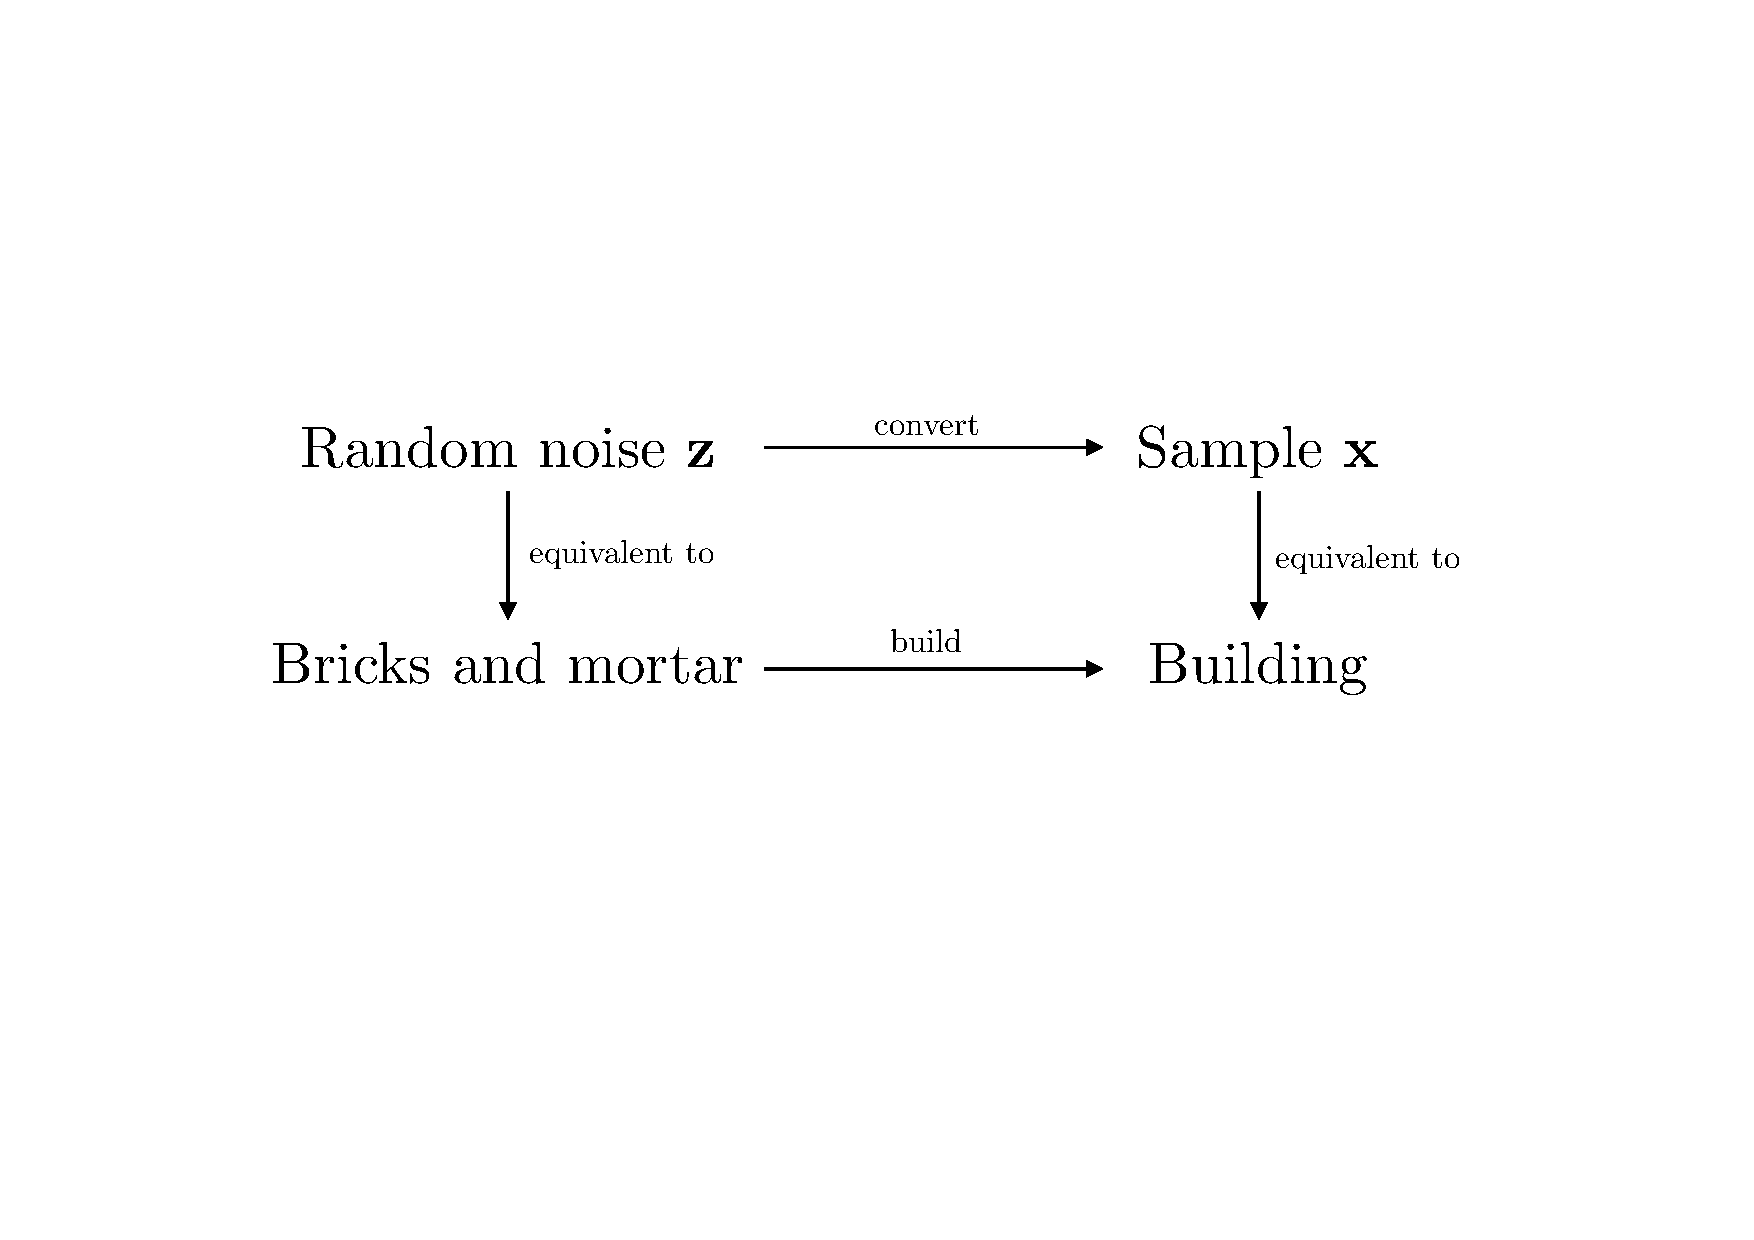
\includegraphics[width=0.5\linewidth]{loop.pdf}
    \caption{Building construction analogy to the DDPM model.}
    \label{fig:analogy}
\end{figure}

We can rethink of the process as a building process, where the noises $\bm{z}$ are the raw materials, in this case, the bricks and mortar, and the samples $\x$  are the final buildings being built. In this case, the generative model becomes the construction team. 

The reconstruction process is bound to be difficult, and this is why there are so many researches involved in the development of generative models. On the other hand, the demolition process is very easy. Considering a \textbf{step-wise process} that gradually demolishing a building into bricks, in this case, let $\x_0$ be the fully-constructed building (initial sample) and $\x_T$ being the fully deconstructed bricks (random noises). Assuming the demolition takes $T$ steps, then the whole demolition process can be written as 
\begin{equation}\label{eq:1.2}
    \x=\x_0\to\x_1\to\x_2\to\cdots \x_{T-1}\to \x_{T}=\bm{z}.
\end{equation}
Within this framework,\marginnote{\footnotesize{\textcolor{red}{It is important to take a note of this at this point, as this is a recurrent trick in the diffusion generative model that tries to learn the reverse construction process. This can be parameterised by any major NN architetures, including convolutional NN, transformer, graph and message-passing NNs for learning atomistic structures. In this regard, diffusion model has very little to do with the designs of the NN but more with the manipulations in the probability distributions of the data.}}} the difficulties in rebuilding a building is that, the jump from the raw materials $\x_T$ to the final building $\x_0$ is too large for a novelist to comprehend how this process can be achieved. However, if we have the intermediate states from the demolition processes $\x_1$, $\x_2$ till $\x_{T-1}$, and we know $\x_{t-1}\to\x_{t}$ represents one small demolition step, then why can't we utilise these information to learn the reverse process $\x_{t}\to\x_{t-1}$ to rebuild the building? This means that if we can learn the relationship between the two \textcolor{red}{$\bmu(\xt)=\xtm$}, then starting from $\x_{T}$, by repetitively applying $\x_{T-1}=\bmu(\x_{T})$,  $\x_{T-2}=\bmu(\x_{T-1})$ and so on, wouldn't we be able to rebuild the whole building $\x_0$?

\subsection{How should we demolish the building?}

Just like we need to eat our meals bite by bite, we also need to rebuild our buildings stepwise. The process of generation in DDPM is actually fully consistent with the the \textbf{analogy of ``demolition followed by reconstruction''} for DDPM. It is a process that first gradually deconstruct the data samples into random noises, then considers a reverse process which is carried out repetitively to (re)generated the (original) new samples. As mentioned before, this is why DDPM is more like a model of \textbf{progressive change} rather than a diffusion model.

More specifically, the demolition process in DDPM takes the following form:
\begin{equation}
    \label{eq:1.3}
    \xt=\alpha_t\x_{t-1}+\beta_t\bm{\varepsilon}_t,\quad\mbox{with}\quad\bm{\varepsilon}_t\sim \mathcal{N}(0,\bm{I}),
\end{equation}
in particular, $\alphat$ and $\betat>0$, $\alphat^2+\betat^2=1$. Usually, we chose $\betat\to0$, it represents how much damage we will make to the building during each step of the demolition process. The introduction of the \textbf{noise} $\et$ represents the destruction to the original signal. We can also think of it as the raw materials, such that in each step of the demolition process, we break $\xtm$ into $\alphat \xtm$ part of the original building plus $\betat\et$ part of the raw materials.

If we repeat the above process, then we have
\begin{align}
\xt&=\alphat\xtm+\betat\et\nonumber\\
&=\alphat\left(\alphatm\bm{x}_{t-2}+\betatm\bm{\varepsilon}_{t-1}\right)+\betat\et\nonumber\\
&=\cdots\nonumber\\
&=(\alphat\alphatm\cdots\alpha_1)\bm{x}_0+\textcolor{red}{(\alphat\alphatm\cdots\alpha_2)\beta_1\bm{\varepsilon}_1+(\alphat\cdots\alpha_3)\beta_2\bm{\varepsilon}_2+\cdots+\betat\et}. \marginnote{\textcolor{red}{\footnotesize{This part is the sum of multiple independent Gaussian noises.}}}\label{eq:1.4}
\end{align}
So why do we require the coefficients must satisfy the constraint $\alphat^2+\betat^2=1$? Let us try to answer this question. In \cref{eq:1.4}, the part that is highlighted in red represents the sum of multiple independent Gaussian noises with the mean of zero, and variances being $(\alphat\alphatm\cdots\alpha_2)\beta_1$, $(\alphat\cdots\alpha_3)\beta_2$, $\ldots$, $\alphat\betatm^2$ and $\betat^2$, respectively. Then, based on the superposition of Gaussians from the probability theory, the sum of Gaussians returns a new Gaussian, which, in the case is of mean zero and variance given by $(\alphat\alphatm\cdots\alpha_2)\beta_1+(\alphat\cdots\alpha_3)\beta_2+\cdots+\betat$. Providing that $\alphat^2+\betat^2=1$, it is not difficult to prove that 
\begin{equation}
    \label{eq:1.5}
(\alphat\alphatm\cdots\alpha_2)\beta_1+(\alphat\cdots\alpha_3)\beta_2+\cdots+\betat=1.
\end{equation}
This means that, effectively, we have \marginnote{\footnotesize{\textcolor{red}{Take note of the definitions $\baralphat=\prod_{i=1}^t\alpha_i$ and $\barbetat=\sqrt{1-\baralphat^2}$, which are commonly used in the diffusion models.}}}
\begin{equation}
    \label{eq:1.6}
\xt=\underbrace{(\alphat\cdots\alpha_1)}_{\equiv\textcolor{red}{\baralphat}}\bm{x}_0+\underbrace{\sqrt{1-(\alphat\cdots\alpha_1)^2}}_{\equiv\textcolor{red}{\barbetat}}\bar{\bm{\varepsilon}}_t,\qquad\bar{\bm{\varepsilon}}_t\sim\mathcal{N}(0,\bm{I}),
\end{equation}
which has now significantly simplified the computations of $\xt$. On the other hand, by choosing a suitable form of $\alphat$ in DDPM to ensure $\baralphat\approx0$ will guarantee that, after $T$ steps of demolitions, the entire building will be fully deconstructed into its raw materials $\bm{\varepsilon}$.

\subsection{How to rebuild the building?}\label{chap_1:rebuild}

During the demolition process $\xtm\to\xt$, we can obtain many pairs of data $(\xtm,\xt)$, therefore, rebuilding is simply a process that learns a model to enable the reverse process $\xt\to\xtm$ to occur. Suppose this model is $\muxt$, then the most straightforward learning protocol is to minimise the Euclidean distance
\begin{equation}
    \label{eq:1.7}
    \|\muxt-\xtm\|_2^2.
\end{equation}
This simple formulation is actually very close to the final DDPM model. Here, we can refine it further. If we first rearrange \cref{eq:1.3} from the demolition process into a reconstructing one by making $\xtm$ the subject:
\begin{equation*}
    \xtm=\frac{1}{\alphat}\left(\xt-\betat\et\right),
\end{equation*}
this then inspires us to express the parameterised reconstruction process analogously as
\begin{equation}
    \label{eq:1.8}
    \muxt=\frac{1}{\alphat}\left(\xt-\betat\bm{\varepsilon}_\theta(\xt,t)\right),
\end{equation}
in which $\theta$ is the learnable parameter. Substituting \cref{eq:1.8} into the loss function \cref{eq:1.7}, we get
\begin{equation}
    \label{eq:1.9}
    \|\muxt-\xtm\|_2^2=\frac{\betat^2}{\alphat^2}\|\et-\bm{\varepsilon}_\theta(\xt,t)\|_2^2.
\end{equation}
Here, $\betat^2/\alphat^2$ represents the weight of the loss function, which we can ignore it for the time being. Substituting  \cref{eq:1.3} and \cref{eq:1.6} for the expression of $\xt$:
\begin{equation}
    \label{eq:1.10}    \xt=\alphat\xtm+\betat\et=\alphat(\alphatmbar\bm{x}_0+\betatmbar\bar{\bm{\varepsilon}}_{t-1})+\betat\et=\alphat\bm{x}_0+\alphat\betatmbar\bar{\bm{\varepsilon}}_{t-1}+\betat\et,
\end{equation}
from which we arrive at a new form of the loss function:
\begin{equation}
    \label{eq:1.11}
    \|\et-\bm{\varepsilon}_\theta(\alphat\bm{x}_0+\alphat\betatmbar\bar{\bm{\varepsilon}}_{t-1}+\betat\et,t) \|_2^2.
\end{equation}
Some readers may wonder why, in \cref{eq:1.10}, we have to go back on step to $t-1$, rather than just go from $t$ to 0 directly? \marginnote{\footnotesize{This process of stepping back one more step will occur recurrently in many derivations in the subsequent chapters.}}
The answer is that, since  we already sampled $\et$ in \cref{eq:1.9}, and $\bar{\bm{\varepsilon}}_t$ is not independent from $\et$, we cannot sample $\bar{\bm{\varepsilon}}_t$ completely as an independent variable, in which case we end up minimising towards a target that is sample dependent.

\subsection{Reducing the square error}\label{sect1:reduce_error}
In principle, we could train DDPM directly using the loss function \cref{eq:1.11}. But in real practice, this is not very tractable, which can lead to slow convergence. This is because \cref{eq:1.11} involves \textbf{four} random variables that can only be obtained through samplings:
\begin{myquote}
\begin{enumerate}
    \item A random sample $\bm{x}_0$ from the inputs.
    \item Sample $\bar{\bm{\varepsilon}}_{t-1}$ and $\bar{\bm{\varepsilon}}_{t}$ from a normal distribution $\mathcal{N}(0,\bm{I})$, giving extra two variables.
    \item Choosing a $t$ from 1 to $T$.
\end{enumerate}
\end{myquote}
The more we need to sample, the more challenge it is to compute the loss function accurately! Fortunately, this problem can be partially mitigated by combining $\et$ and $\bar{\bm{\varepsilon}}_{t-1}$ into a single random variable sampled from a normal distribution using the integration trick. Because the product of two normal distributions is still a normal distribution, so we have $\alphat\betatmbar\bar{\bm{\varepsilon}}_{t-1}+\betat\et$ is equivalent to $\betatbar\bm{\varepsilon}|\bm{\varepsilon}\sim\mathcal{N}(0,I)$. Equally, we have \textcolor{blue}{$\betat\bar{\bm{\varepsilon}}_{t-1}-\alphat\betatmbar\et$ that is equivalent to $\betatbar\bm{w}|\bm{w}\sim\mathcal{N}(0,I)$}.\marginnote{\footnotesize{\textcolor{blue}{Not quite sure where this comes from?}}} Furthermore, it can be proven that $\mathbb{E}[\bm{\varepsilon}\bm{w}^T]=0$, so they are two independent normal distributions. With this, we can express $\et$ with $\bm{\varepsilon}$ and $\bm{w}$:
\begin{equation}
    \label{eq:1.12}
    \et=\frac{(\betat\bm{\varepsilon}-\alphat\betatmbar\bm{w})\betatbar}{\betat^2+\alphat^2\betatmbar^2}=\frac{\betat\bm{\varepsilon}-\alphat\betatmbar\bm{w}}{\betatbar}.
\end{equation}
Substitute \cref{eq:1.12} into \cref{eq:1.11}, we get
\begin{align}
    &\mathbb{E}_{\bar{\bm{\varepsilon}}_{t-1},\et\sim\mathcal{N}(0,\bm{I})}\left[\left\| \et-\bm{\varepsilon}_\theta(\alphat\bm{x}_0+\alphat\betatmbar\bar{\bm{\varepsilon}}_{t-1}+\betat\et,t) \right\|_2^2\right]\nonumber\\
    &=\mathbb{E}_{\bm{w},\bm{\varepsilon}\sim\mathcal{N}(0,\bm{I})}\left[\left\| \frac{\betat\bm{\varepsilon}-\alphat\betatmbar\bm{w}}{\betatbar}-\bm{\varepsilon}_\theta (\alphatbar\bm{x}_0+\betatbar\bm{\varepsilon},t)   \right\|_2^2 \right]. \label{eq:1.13}
\end{align}
Note that the loss function is quadratic in $\bm{w}$, which we can expand the square and then determine the expectation value, this gives,
\begin{equation}
    \label{eq:1.14}
    \frac{\betat^2}{\betatbar^2}\mathbb{E}_{\bm{\varepsilon}\sim\mathcal{N}(0,\bm{I})}\left[\left\| \bm{\varepsilon}-\frac{\betatbar}{\betat}\bm{\varepsilon}_\theta (\alphatbar\bm{x}_0+\betatbar\bm{\varepsilon},t)   \right\|_2^2 \right]+\mathcal{C}.
\end{equation}
Ignoring the weight and constant again, we arrive at:\marginnote{\footnotesize{\textcolor{red}{This basically says, we must first sample a noise from the normal distribution $\mathcal{N}(0,\bm{I})$, from which we can generate the noisy sample $\xt=\alphatbar\bm{x}_0+\betatbar\bm{\varepsilon}$. Then we plug this $\xt$ into the denoising network $\bm{\varepsilon}_\theta(\xt)$ to recover $\et$. This expression is equivalent to the results\cite{luo2022understanding} derived using KL divergence between the destruction and regeneration process: $\argmin_\theta\mathcal{D}_{KL}(q(\xtm|\xt,\bm{x}_0)$ $\|p(\xtm|\xt))$ from evidence lower bound, which upon further reparameterisation, gives the following expression for the KL divergence: $\frac{(1-\alphat)^2}{2\sigma_q^2(t)}\frac{\|\bm{\varepsilon}_0-\hat{\bm{\varepsilon}}_\theta(\bm{x},t)\|_2^2}{(1-\alphatbar)\alphat}$.}}}
\textcolor{red}{
\begin{equation}\label{eq:1.15}
    \mathbb{E}_{\bm{\varepsilon}\sim\mathcal{N}(0,\bm{I})}\left[\left\| \bm{\varepsilon}-\frac{\betatbar}{\betat}\bm{\varepsilon}_\theta (\alphatbar\bm{x}_0+\betatbar\bm{\varepsilon},t)   \right\|_2^2 \right],
\end{equation}}
which is the final form of the lost function for DDPM.

\subsection{Regressive generations}
Above, we have clarified the training procedures for DDPM. The derivation is a bit lengthy and not immediately trivial. While it is not easy to understand, it is not totally difficult either, since it has not applied the mathematical tools that are needed in the traditional diffusion models, but only an analogous model of building demolition and reconstruction plus some basic knowledge in the probability theory. As such, this newly formulated diffusion generated model, as represented by DDPM, is not as mathematically complicated as one may think. 

After the model is being trained, we can perform samplings to generate new samples. Starting from a random noise $\bm{x}_T\sim\mathcal{N}(0,\bm{I})$, and repeat the process for $T$ steps according to \cref{eq:1.8}:
\begin{equation}
    \label{eq:1.16}
    \xtm=\frac{1}{\alphat}(\xt-\betat\bm{\varepsilon}_\theta(\xt,t)).
\end{equation}
This corresponds to the \textbf{greedy search} in VAE. For random sampling, we can add an additional noise term:
\begin{equation}
    \label{eq:1.17}
    \xtm=\frac{1}{\alphat}(\xt-\betat\bm{\varepsilon}_\theta(\xt,t))+\sigma_t \bm{z}\qquad \bm{z}\sim\mathcal{N}(0,\bm{I}).
\end{equation}
In practice, \textcolor{red}{we can keep $\betat=\sigma_t$}, i.e., the variances are the same for both the forward and reverse diffusions.

It should be noted that the sampling process in DDPM is different from the one performed with Langevin equation. In DDPM, each sampling process starts from a new random noise, and is iterated for $T$ steps to generate a new sample. On the other hand, Langevin sampling starts from a single random point and iterates definitively. In principle, all samples can be generated through infinite iterations. Therefore, although DDPM shares similarity with the Langevin sampling, they are fundamentally different models.

\subsection{Hyperparameter settings}
In DDPM, the upper limit $T$ is usually set to 1000, which is much larger than what people usually expect. Why such a large value is necessary? In the original publication, the following function is used to set $\alphat$:
\begin{equation}
    \label{eq:1.18}
    \alphat=\sqrt{1-\frac{0.02t}{T}},
\end{equation}
which is a monotonically decreasing function. Why such a choice is also necessary?

The above two questions are inter-dependent, and is related to the nature of the data. When the Euclidean distance is used for constructing the loss function, experience of image reconstructions using VAE shows that, only when the input and output images are sufficiently close to each other, we can generate new images of higher quality. Thus, using large time can make sure the input and output in each time step are sufficiently similar to each other, reducing the blurring effects from using the Euclidean distance in the loss function. 

A similar reason applies to  the choice of a monotonically decreasing function for $\alphat$. When $t$ is small, $\xt$ is close to the real image, so we need to decrease the distance between $\xtm$ and $\xt$, making it more suitable to apply the Euclidean distance in \cref{eq:1.7}. This gives large $\alphat$. When $t$ is very large, $xt$ becomes very close to a true Gaussian noise, which can be modelled with the Euclidean distance, thus we can increase the distance between $\xtm$ and $\xt$ with smaller $\alphat$. Can we use a large $\alphat$ throughout the forward process then? In principle the answer is yes, but we need to increase $T$. Recall that when we derived \cref{eq:1.6}, we wanted $\bar{\alpha}_T\approx0$, which we can evaluate
\begin{equation}
    \label{eq:1.19}
    \log\bar{\alpha}_T=\frac{1}{2}\sum_{t=1}^T \log \left( 1-\frac{0.02t}{T}\right) < \frac{1}{2}\sum_{t=1}^T \log \left(-\frac{0.02t}{T}\right)=-0.005(T+1)
\end{equation}
With $T=1000$, $\bar{\alpha}_T\approx 10^{-5}$, which is nearly zero as we wished. As a result, if we want to use a large $\alpha_t$ throughout, then we will have to increase $T$.

Finally, note that in the loss function [\cref{eq:1.15}, $\bm{\varepsilon}_\theta(\alphatbar\bm{x}_0+\betatbar\bm{\varepsilon},t)$], the time variable $t$ has been explicitly included. This is because, at different $t$, we are dealing with data of different noise levels. Therefore, \textbf{we are required to have $T$ different reconstruction models}, meaning \textbf{$T$ is also a model hyperparameter}.